Population dynamics is about populations changing in numbers. Populations may be age-structured (common in human demographic models), stage-structured (\eg\ insects or plants), size-structured (\eg\ fish or trees) or otherwise structured. When populations are modelled, we must consider what detail of structure is necessary to capture the essential dynamics.

In simulations, populations are often initialised with some initial density or population size at time zero with no specific reference to a calendar. However, for many populations it is important to model the phenology of life stages through the seasons of the year. Getting the phenology right is a good first step when modelling population dynamics.

\section{A butterfly model}
\subsection{Phenology}
The model below simulates the stage-structured phenology of a butterfly population (box script from \filenameexplained{book/butterfly1.box}).

\lstset{numbers=left}
\begin{boxscript}
// butterfly1.box
Simulation sim {
  .steps = 273
  Calendar calendar {
    .initialDateTime = 1/5/2009
  }
  Records weather {
    .fileName = "weather/flakkebjerg 2009.txt"
  }
  Box butterfly {
    Stage egg {
      .initial = 100 
      .duration = 140
      .timeStep = ./time[step]
      DayDegrees time {
        .T0 = 5
        .T = weather[Tavg]
      }
    }
    Stage larva {
      .inflow = ../egg[outflow]
      .duration = 200
      .timeStep = ./time[step]
      DayDegrees time {
        .T0 = 8
        .T = weather[Tavg]
      }
    }
    Stage pupa {
      .inflow = ../larva[outflow]
      .duration = 100
      .timeStep = ./time[step]
      DayDegrees time {
        .T0 = 10
        .T = weather[Tavg]
      }
    }
    Stage adult {
      .inflow = ../pupa[outflow]
      .duration = 28
      .timeStep = 1
    }
  }
  OutputR {
    PageR {
      .xAxis = calendar[date]
      .ncol = 2
      PlotR {
        .ports = *[content]
        .ggplot = "scale_x_datetime(
                     breaks = date_breaks('months'), 
                     labels = date_format('%\%%b')
                   )" 
      }
      PlotR {
        .ports = *[outflowTotal]
        .ggplot = "scale_x_datetime(
                     breaks = date_breaks('months'), 
                     labels = date_format('%\%%b')
                   )" 
      }
    }
  }
}
\end{boxscript}
\lstset{numbers=none}

You will recognize pieces of code also found in the egg development model, that we worked on earlier (\filename{\inputfolder/book/egg5.box}). The previous egg model is embedded  in lines 11-19, including its day-degree model. The familiar sequence of four life stages (egg-larva-pupa-adult) has been stringed together setting the \code{inflow} port of one life stage to the \code{outflow} port of the previous life stage (lines 21, 30, 39). The egg stage, being the initial life stage, has no inflow but rather an \code{initial} number set to 100 (line 12). The model follows the development of these 100 individuals, starting as eggs and ending their life dying of old age as adults; the \code{outflow} from the \code{adult} model is used nowhere and is thus silently lost.

The four life stages work on different time scales as set by their \code{timeStep} inputs (lines 14, 23, 32 and 41). Notice how for the first three life stages, the \code{timeStep} is set to the same expression:
\begin{boxscript}
.timeStep = ./time[step]
\end{boxscript}

Logically, they refer to the same port: the \code{step} port of its \code{time} child model (for the meaning of the dot in \code{./time}, see \iref{ch:path-expressions-dot}). However, since they each have a different \code{time} child model, their time scales will differ. Moreover, their durations differ as well (lines 13, 22 and 31). The adult life stage works more simply on a physical time scale, spending 1 day per time step (line 41) with a duration of 28 days (line 40).

The output consists of two plots (lines 48-54 and 55-61) arranged side by side, as set by \code{ncol} (line 47). The plot \code{ports} are both set with a joker (\iref{ch:path-expressions-jokers}) for the box name (line 49 and 57) which resolves to four ports shown in both plots, one port for each life stage.

In R the plots are produced by the \concept{ggplot} package. You can modify the default plot through the \code{ggplot} input to the \code{PlotR} box. The R code written here will be added to the ggplot. Here the plots are augmented by the \code{scale_x_datetime} R function to produce monthly breaks on the \xaxis\ (lines 50-53 and 57-60). The ggplot package offers a lot of liberty in how plots are constructed. Any specific solution can usually be found quickly on Internet; that is how I found this particular one.

Real programmers will scoff at our code due to the replication of code in lines 50-54 and 58-62. Experience has taught programmers that code without replication is easier to read and maintain. Here is how to fix that (in \filename{butterfly2.box}):

\lstset{numbers=left}
\begin{boxscript}
OutputR {
  PageR {
    .xAxis = calendar[date]
    .ncol = 2
    &monthBreaks = "scale_x_datetime(
                      breaks = date_breaks('months'), 
                      labels = date_format('%\%%b')
                    )" 
    PlotR {
      .ports = *[content]
      .ggplot = ..[monthBreaks]
    }
    PlotR {
      .ports = *[outflowTotal]
      .ggplot = ..[monthBreaks]
    }
  }
} 
\end{boxscript}
\lstset{numbers=none}

It turns out that we are allowed to create new ports in box scripts. They are called \concept{blind ports} because you cannot see them in the original \CPP\ code. You declare a blind port by preceeding it with an ampesand (\code{&}) rather than a dot (\code{.}). Here we declared \code{monthBreaks} (lines 5-8) to hold the common code and then refer to that port when setting the two \code{ggplot} inputs (lines 11 and 15); the double-dots (\code{..}) refer to the parent box (\iref{ch:path-expressions-double-dot}). Programmers will recognise that blind ports can work like local variables, as found in many other programming languages. In contrast to local variables, however, blind ports -- like other ports -- can be read from any box in the script by reference to the box containing the port. So, all ports have a local anchorage by the box owning them but can be used globally.

\begin{figure} [ht]
\centering
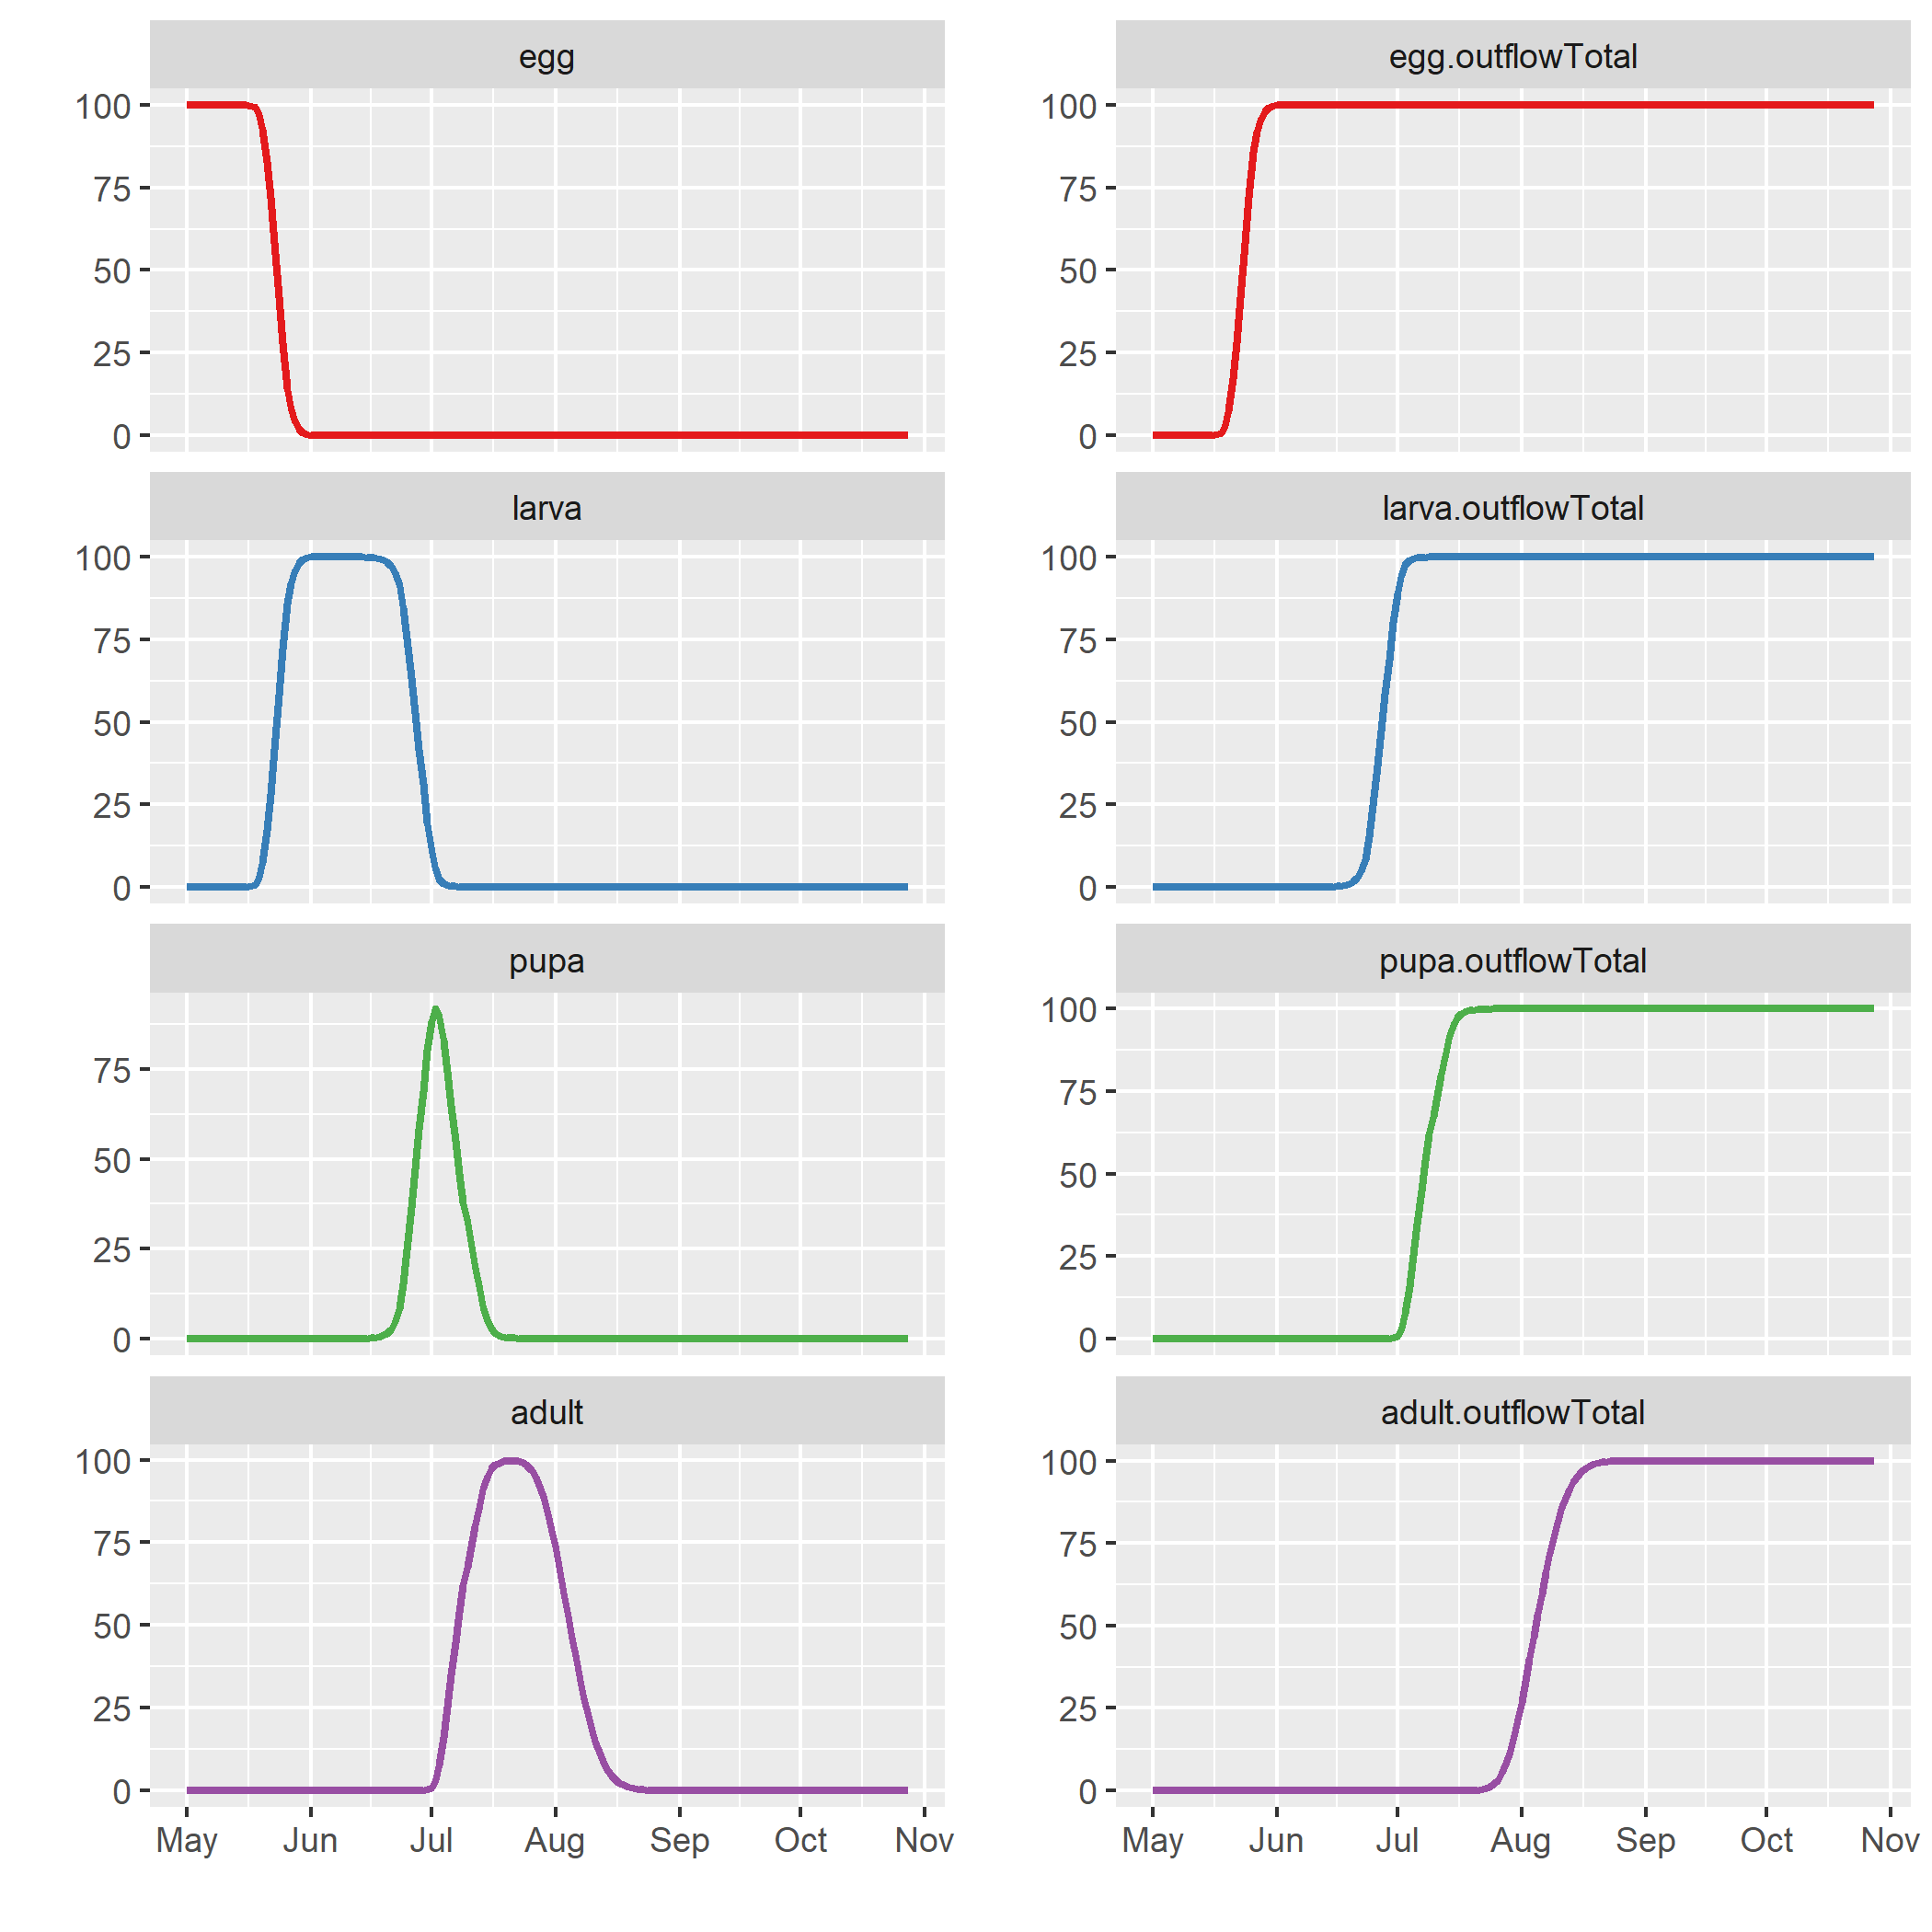
\includegraphics[width=\textwidth]{graphics/butterfly2}
\caption{Life stage phenology produced by both \filename{\inputfolder/book/butterfly1.box} and \filename{\inputfolder/book/butterfly2.box}.}
\label{fig:butterfly2}
\end{figure}

In the output (\iref{fig:butterfly2}), the \code{content} and \code{outflowTotal} ports are shown on the left and right side, respectively. The initial 100 eggs can be followed as they hatch and trickle through the subsequent life stages. The adults fly in the first half of August. We note that the effort to produce an \xaxis\ with nice monthly breaks paid off.

\subsection{Reproduction}
The butterfly species we are simulating is hypothetical. Let's say that it has one generation per year, and that it overwinters in the egg stage. Moreover, let's assume that upon emerging from the pupa, a female spends 5 days in a pre-oviposition stage before laying eggs during the following 10 days. Presumable, the last 13 days of its 28 days total life span, it spends just being pretty. Finally, let's assume that the net reproductive rate ($R_0$) for a female is 80. With an assumed sex ratio of 0.5 that means $R_0=40$ for an average individual.

To achieve multiplication of individuals in our model, we will use yet another feature of the distributed delay model. Originally identified by the 'attrition' parameter of the distributed delay \citep{Vansick77}, in the \code{Stage} class it is managed through the \code{growthFactor} port (\iref{ch:physiological-development-stage}). 

The effect of \code{growthFactor} is deceptively simple. If we use $\lambda$ as a shorthand for \code{growthFactor} then for every unit $\Delta x$ that enters the \code{Stage} box (through its \code{inflow} port), eventually $\lambda\Delta x$ units will leave the box (through its \code{outflow} port and accumulated in its \code{outflowTotal} port). The value of \code{growthFactor} may vary through the simulation but it must always be larger than zero. Its default value is 1. Wherein lies the deception? Despite the explanation being no longer than what you have just read, users of the distributed delay and hence users of the \code{Stage} class routinely get confused. You have been warned.

We implement reproduction, replacing the \code{adult} box found in \filename{\inputfolder/book/butterfly2.box} with the code below. The updated box script can be found in \filename{\inputfolder/book/butterfly3.box}.

\lstset{numbers=left}
\begin{boxscript}
// From butterfly3.box
Box adult {
  Stage adult {
    .inflow = ../../pupa[outflow]
    .duration = 28
    .timeStep = 1
  }
  Stage preOviposition {
    .inflow = ../../pupa[outflow]
    .duration = 5
    .timeStep = 1
  }
  Stage oviposition {
    .inflow = ../preOviposition[outflow]
    .duration = 10
    .timeStep = 1
    .growthFactor = 40
  }
}
\end{boxscript}
\lstset{numbers=none}

In the new model, the adult life stage is simulated by three \code{Stage} boxes rather than just one. To keep them nicely together, the three \code{Stage} boxes have been nested inside a box aptly called \code{adult} (line 3). This box simply acts as a container for the other boxes, so it is of the generic \code{Box} class. \CPP\ programmers will appreciate that \code{Box} is the base class for all box classes in the \US\ framework.

The first \code{Stage} (lines 3-7) holds the adults proper and remains unchanged from the previous version of the box script. For want of a better name, it is called \code{adult} as well. Second comes \code{preOviposition} (lines 8-12). Note that it parallels the adult stage, as they both take the \code{outflow} from the pupa stage as \code{inflow} (lines 5 and 10). The \code{preOviposition} box is used to keep track of how many individuals are in the pre-oviposition stage.

Finally, the \code{oviposition} box (lines 13-18) keeps track of the egg-laying process. The number of eggs laid every day will show in the \code{outflow} port of the \code{oviposition} box. The accumulated number of eggs laid will show in its \code{outflowTotal} port. The multiplication is achieved through \code{growthFactor} which has been set to 40 (line 18). Hence for every individual that enters, 40 individuals will exit. In a sense this is true; by oviposition every adult is converted into 40 eggs. Since 100 individuals enter in total, we expect 4,000 eggs to be laid in total. This is exactly what we find in the simulation output (\iref{fig:butterfly3}).
 
\begin{figure}
\centering
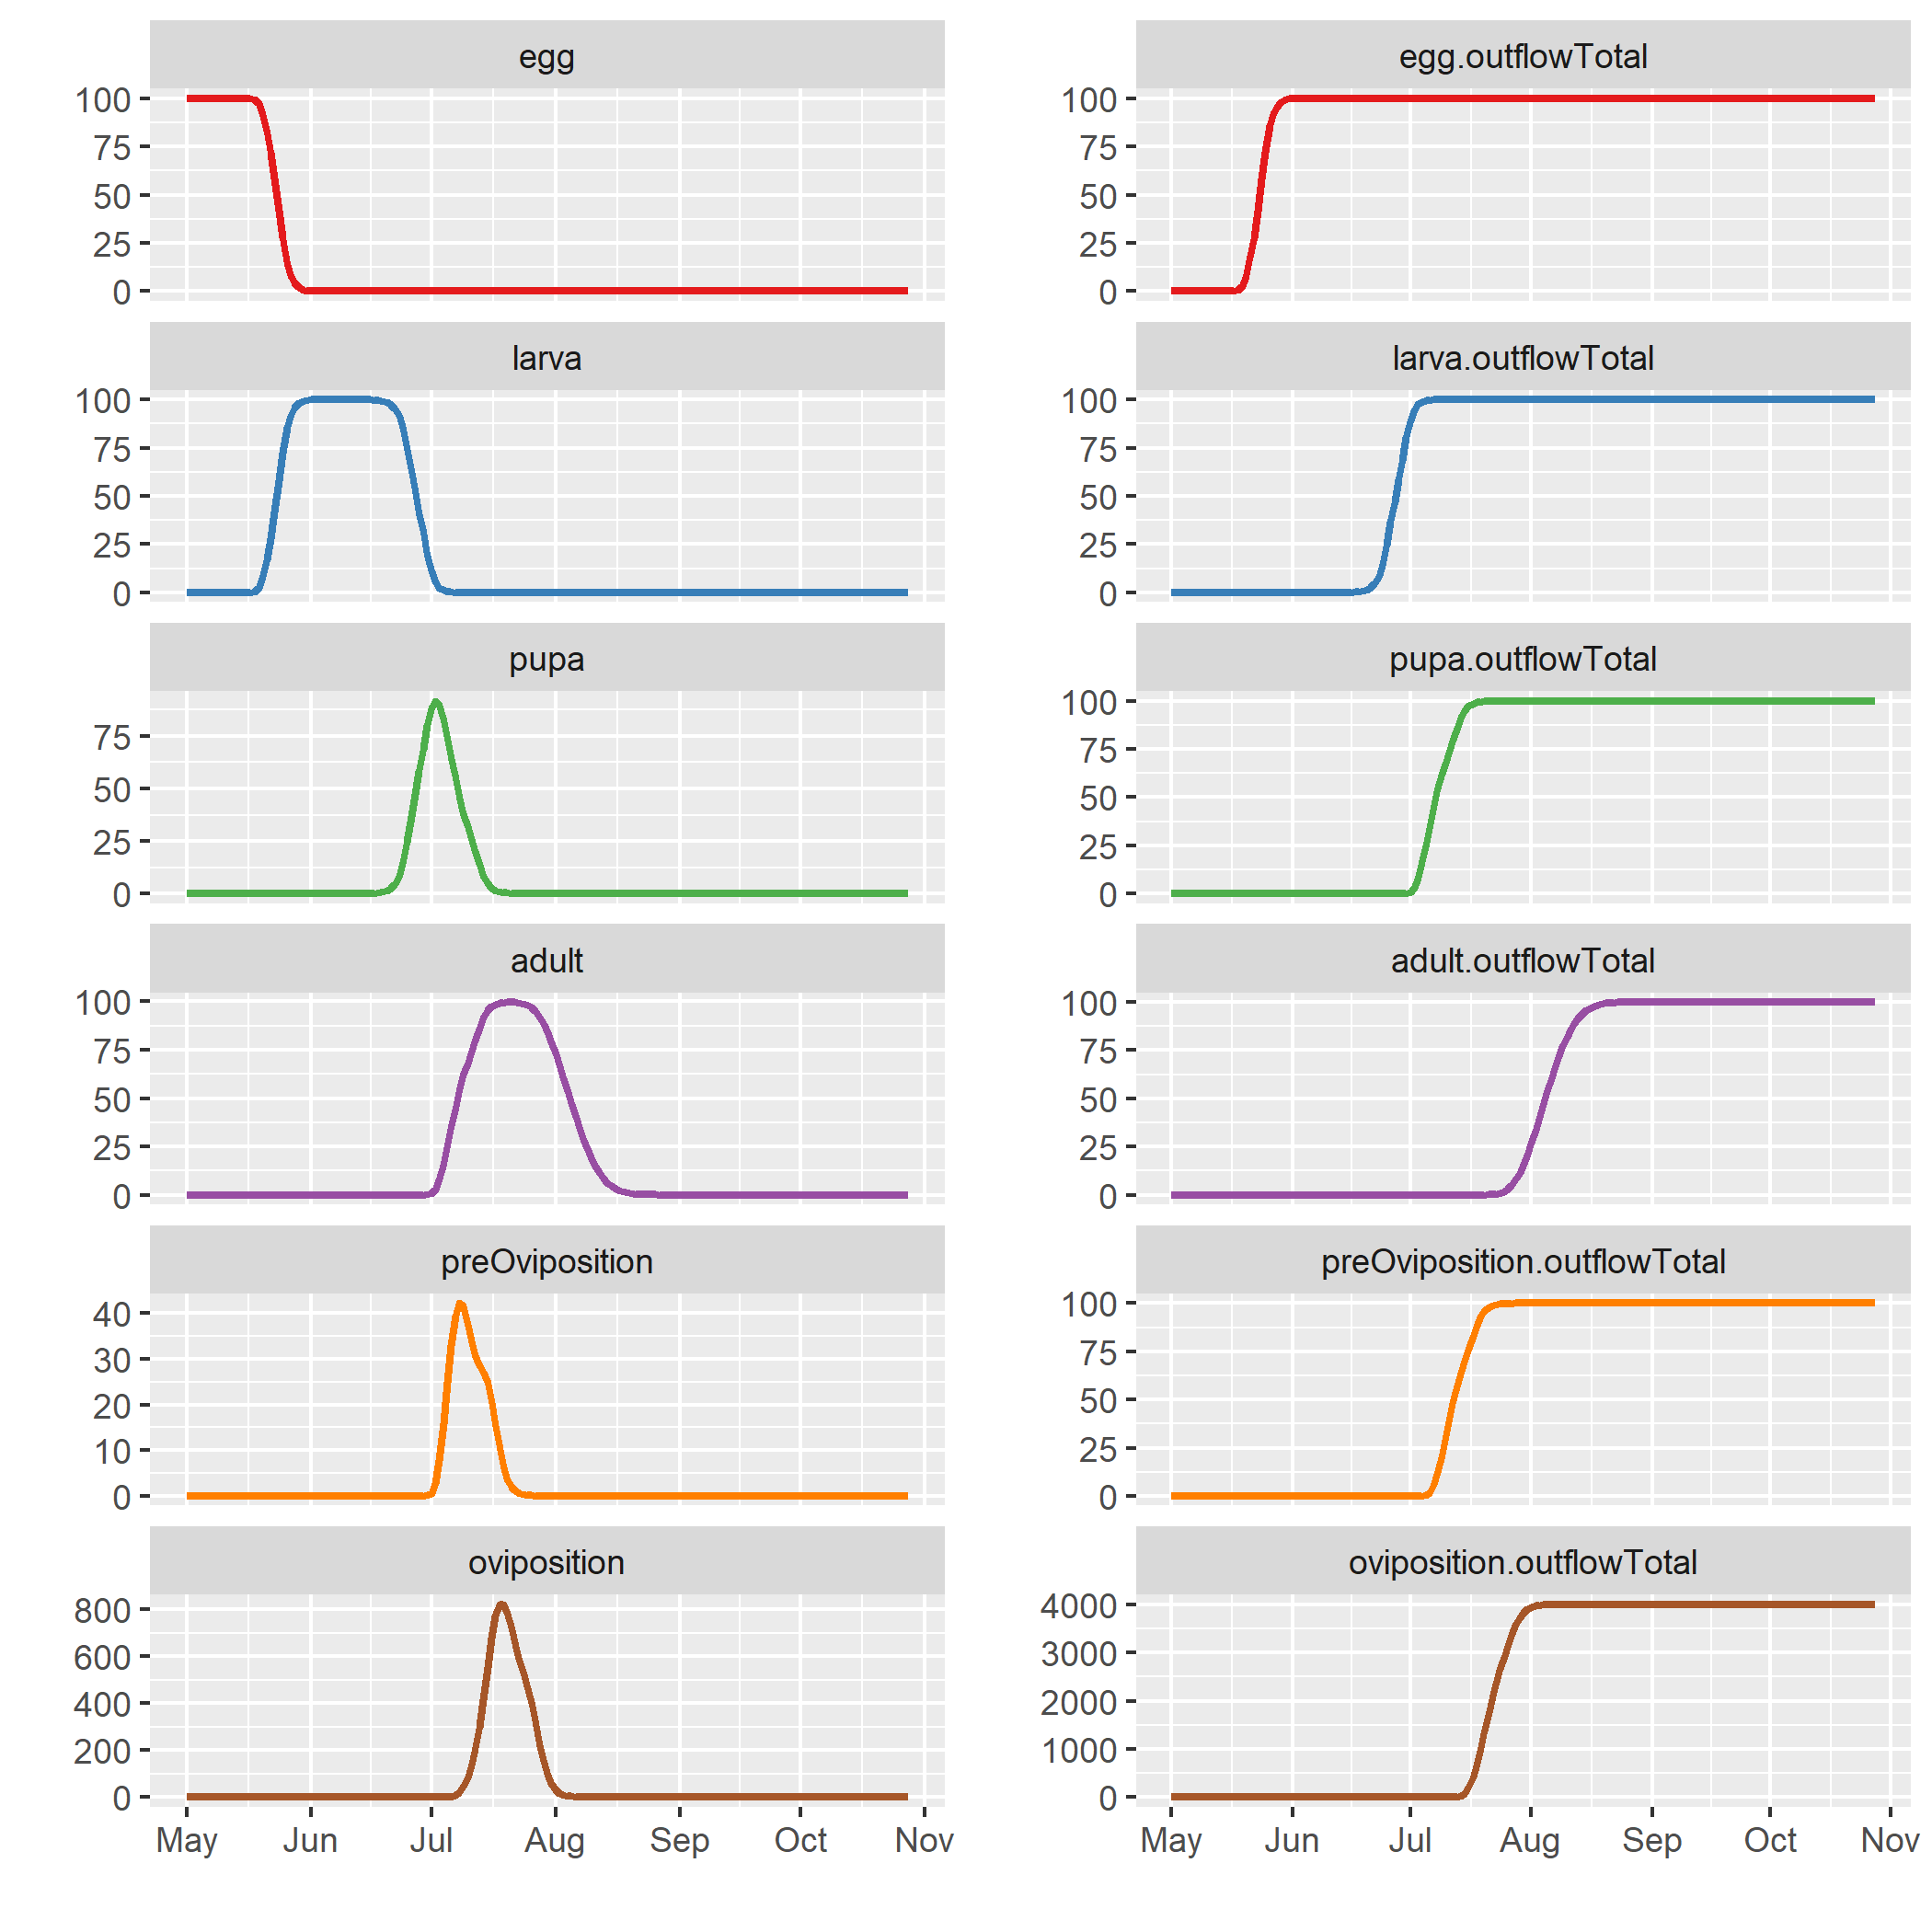
\includegraphics[width=\textwidth]{graphics/butterfly3}
\caption{Life stage and oviposition phenology produced by the \filename{\inputfolder/book/butterfly3.box} script.}
\label{fig:butterfly3}
\end{figure}

If you want to study the simulation output in further detail, you can see the exact numbers in R. All the outplut displayed as plots comes from an R data frame called \code{sim}. Write \rcom{sim} at the R prompt to see it all speeding by and fill up your screen, or better, type \rcom{tail(sim)} to see just the final rows. You can then verify that, indeed, the \code{oviposition.outflowTotal} column has reached a value of 4,000 in the last row.

\subsection{Multiple years}
As a final touch to the butterfly model, we will enable it to run for multiple years. Because we have included no mortality factors in the model, we expect the population to multiply by a factor of $R_0=40$ per year. But first we need to fix some shortcuts that we took in the one-year model.

\subsubsection{Restrict egg development}
The one-year model simulates the population from 1 May until an arbitrary date in autumn. To prepare the model to run for many years, it should run from 1 January to 31 December. At first we chose 1 May as a starting date, just because that is when we start computing day-degrees for egg development. If we change the starting date to 1 January,
\begin{boxscript}
Calendar calendar {
  .initialDateTime = 1/1/2009 
}
\end{boxscript}
then eggs will start development too early in the year. Biologically, the period of egg development could be restricted by day length or some other mechanism, that we have not included in the model.

To restrict egg day-degrees to accumulate from 1 May only, we must make some changes to the \code{egg} model:

\lstset{numbers=left}
\begin{boxscript}
// From butterfly4.box
Stage egg {
  .initial = 100 
  .inflow = ../adult/adult/oviposition[outflow] 
  .duration = 140
  .timeStep = ./time[value] 
  OnOff time { 
    .x = calendar[dayOfYear]
    .xOn = 107    // 17 April
    .xOff = 152   //  1 June
    .valueOn = ./dayDegrees[step]
    .valueOff = 0
    DayDegrees dayDegrees {
      .T0 = 5
      .T = weather[Tavg]
    }
  }
}
\end{boxscript}
\lstset{numbers=none}

Here, we have used an \code{OnOff} box which sets its output \code{value} to \code{valueOn} (line 11) inside a certain \code{x} interval and to \code{valueOff} (line 12) outside the \code{x} interval. For \code{x} we use the day of the year, which we get from \code{calendar} (line 8). With \code{xOn} and \code{xOff} we limit the interval to $[107,152]$, \ie\ from 17 April  to 1 June (lines 9-10). Note, how \code{valueOn} in line 11 refers to the \code{dayDegrees} box, which  has not changed (lines 13-16).

With egg development restricted in time, we are ready to transfer the eggs laid (by the \code{oviposition} box) into the \code{egg} box. This is taken care of in line 4. Note the rather deep reference \code{../adult/adult/oviposition[outflow]}. We could have written this much shorter, as \code{oviposition[outflow]}, since there is only one match in this box script to this path. However, as a rule you write more robust box scripts by using local references (\ie\ those beginning with a dot or double-dot). If you later were to add another population to this box script, which also had an \code{oviposition} box inside it, then the local reference in line 4 would still match the one and same port, whereas \code{oviposition[outflow]} would match two ports (and cause an error message).

The output from the improved model (\iref{fig:butterfly4}) has been extended with an additional column to show how the new logic for egg development works. From the top: the day of the year, ambient temperature, daily day-degrees above the the temperature threshold for eggs, the period when egg development is on, and lastly the resulting day-degrees accrued daily by the eggs. To make room for the \xaxis\ labels, the ggplot code has been changed to break for every 3 months instead of every month (see how in the \filename{butterfly4.box} script, or just below in \filename{butterfly5.box}).

\begin{figure}
\centering
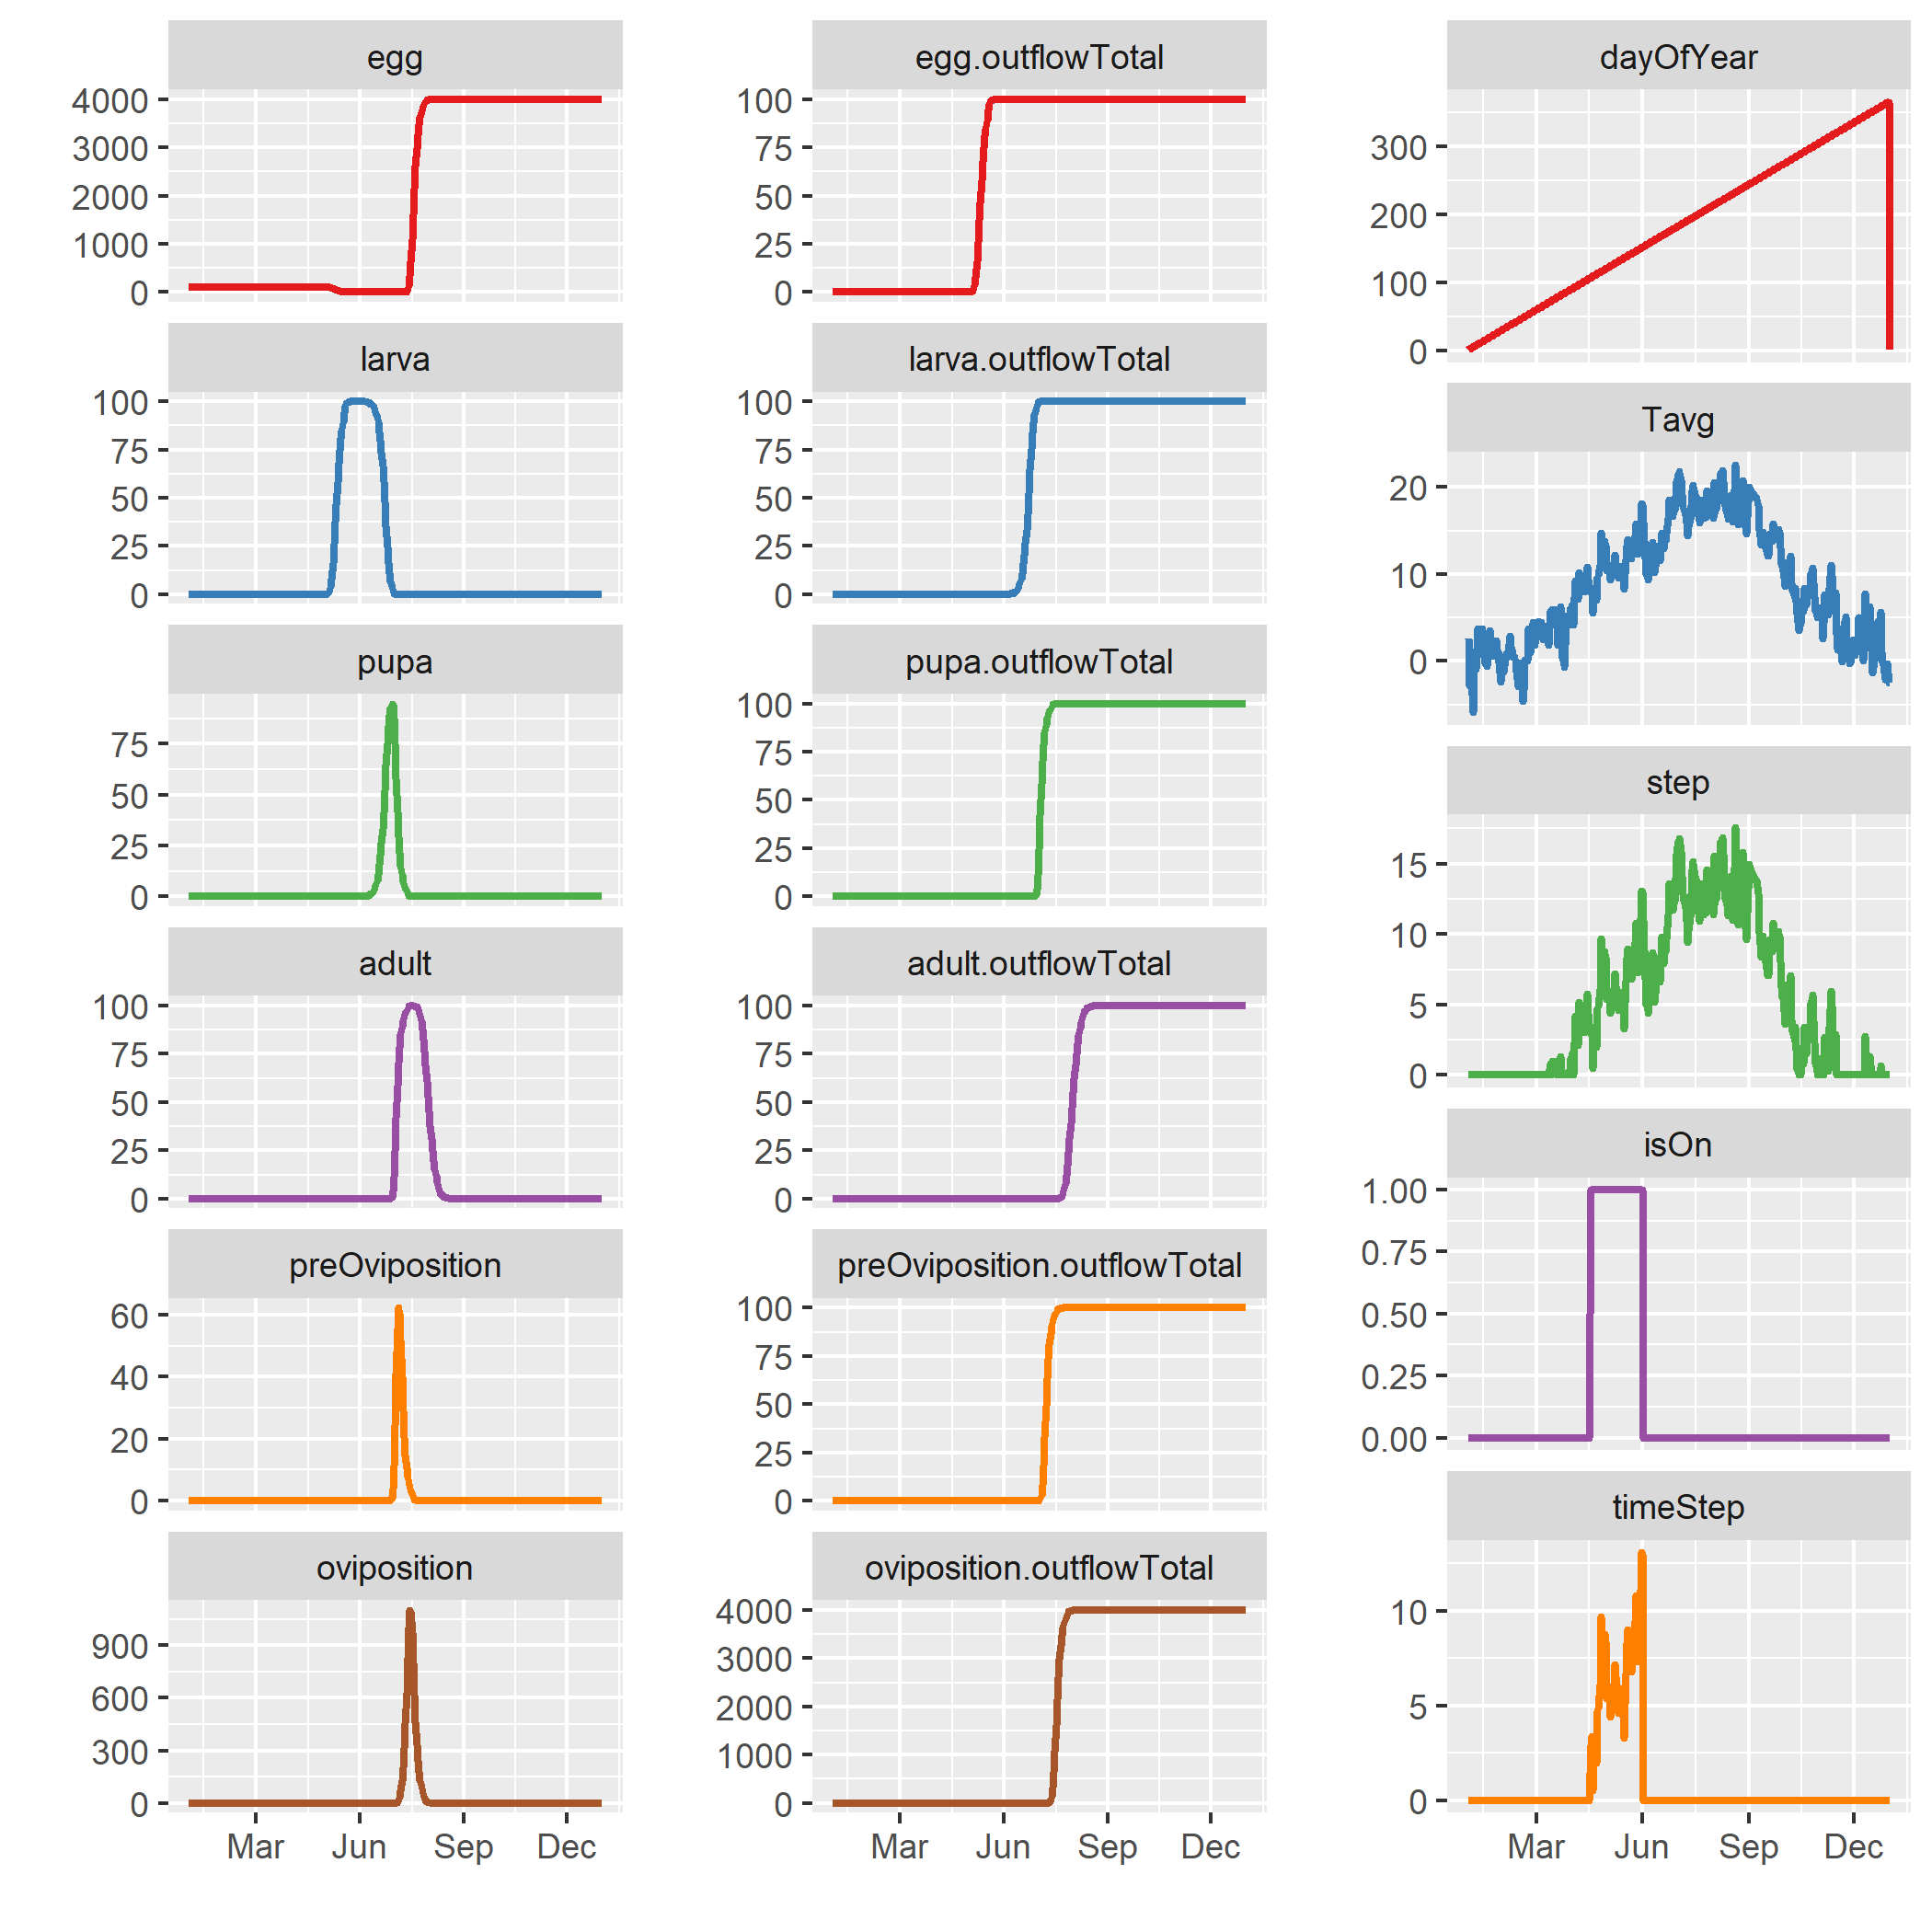
\includegraphics[width=\textwidth]{graphics/butterfly4}
\caption{Life stage and oviposition phenology (left and mid column), together with logic for egg development (right column). Produced by the \filename{\inputfolder/book/butterfly4.box} script.}
\label{fig:butterfly4}
\end{figure}

\subsubsection{Transform \yaxis}
To be prepared for the large numbers expected, when we run the model for more than one year, we change the \yaxis\ scale to show $log_{10}$-transformed numbers. We make the following changes inside the \code{PageR} box:

\lstset{numbers=left}
\begin{boxscript}
// From butterfly5.box
&monthBreaks = "scale_x_datetime(
                  breaks = date_breaks('3 months'), 
                  labels = date_format('%\%%b')
                ) + 
                ylim(0,NA)" 
PlotR {
  .ports = *[content]
  .ggplot = ..[monthBreaks]
  .transform = "log10" 
}
PlotR {
  .ports = *[outflowTotal]
  .ggplot = ..[monthBreaks]
  .transform = "log10" 
}
\end{boxscript}
\lstset{numbers=none}

For the two plots showing populations numbers, we set the \code{transform} input to \code{log10} (lines 11 and 16). On its own, however, this change brings about big negative numbers, as population numbers tend toward zero. So, in addition, we set the lower limit of the \yaxis\ to 0 (line 7). In effect, population densities below 1 (since $log(1)=0$) will be omitted from the plots. In comparison to the previous version (\iref{fig:butterfly4}), we can now more easily read graphs spanning large numerical ranges, \eg\ the eggs starting on 100 and ending on 4,000 (\iref{fig:butterfly3b}).

\begin{figure} [h]
\centering
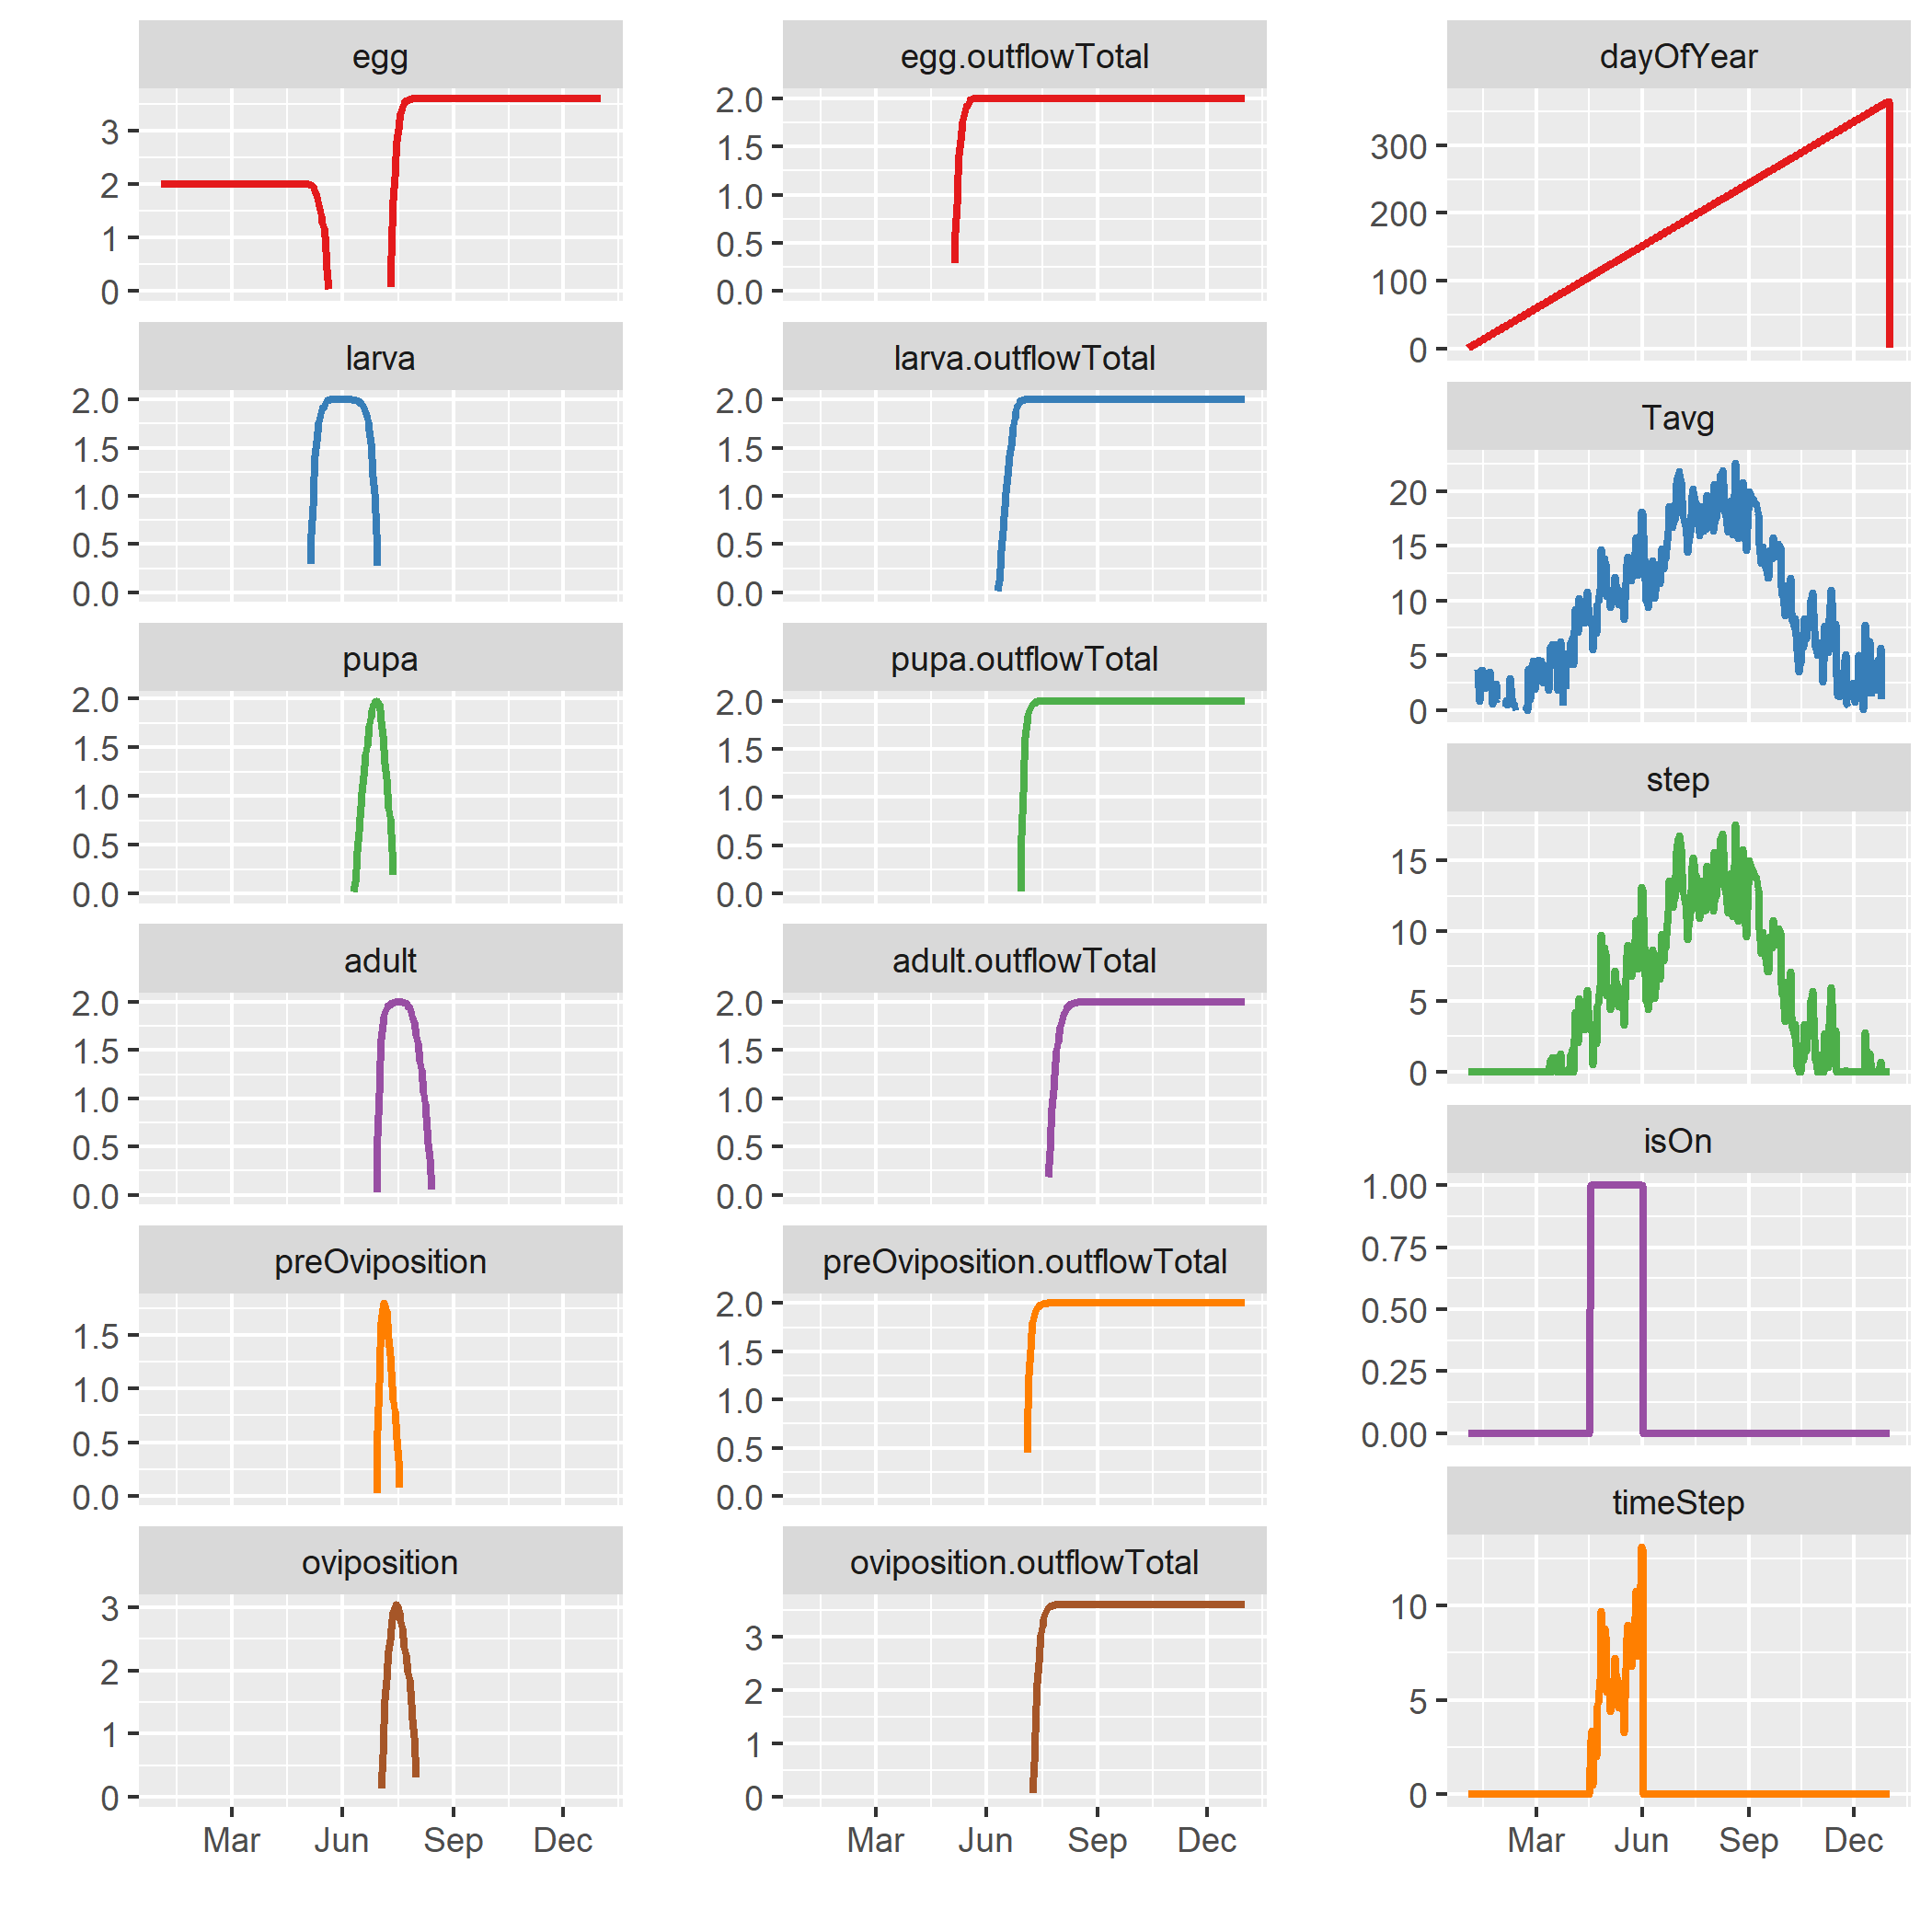
\includegraphics[width=\textwidth]{graphics/butterfly5}
\caption{Egg numbers on a $log_{10}$-scale. Produced by the \filename{\inputfolder/book/butterfly5.box} script.}
\label{fig:butterfly5}
\end{figure}

\subsubsection{Cycle through years}

To let the model run for 3 years, we must to change the number of simulation steps to account for 1,085 days (line 3):

\lstset{numbers=left}
\begin{boxscript}
// From butterfly6.box
Simulation sim {
  .steps = 1085 
  Calendar calendar {
    .initialDateTime = 1/1/2009 
  }
  Records weather {
    .fileName = "weather/flakkebjerg 2009.txt"
    .cycle = TRUE
  }
  :
}
\end{boxscript}
\lstset{numbers=none}

However, we have only got weather data for one year (2009). To re-use these data for every year, we tell the \code{Records} box that is should \code{cycle} through the weather file again and again (line 9). You can find the full script for the final model in  \filename{\inputfolder/book/butterfly6.box} with \xaxis\ breaks enlarged from 3 months to 4 months. The output is as expected (\iref{fig:butterfly6}). Moreover, if you type \rcom{tail(sim)} at the R prompt, you will see that the final egg population (in the \code{egg.content} column) is as expected, namely $100{R_0}^3=100\cdot40^3=6,400,000$.


\begin{figure} [b]
\centering
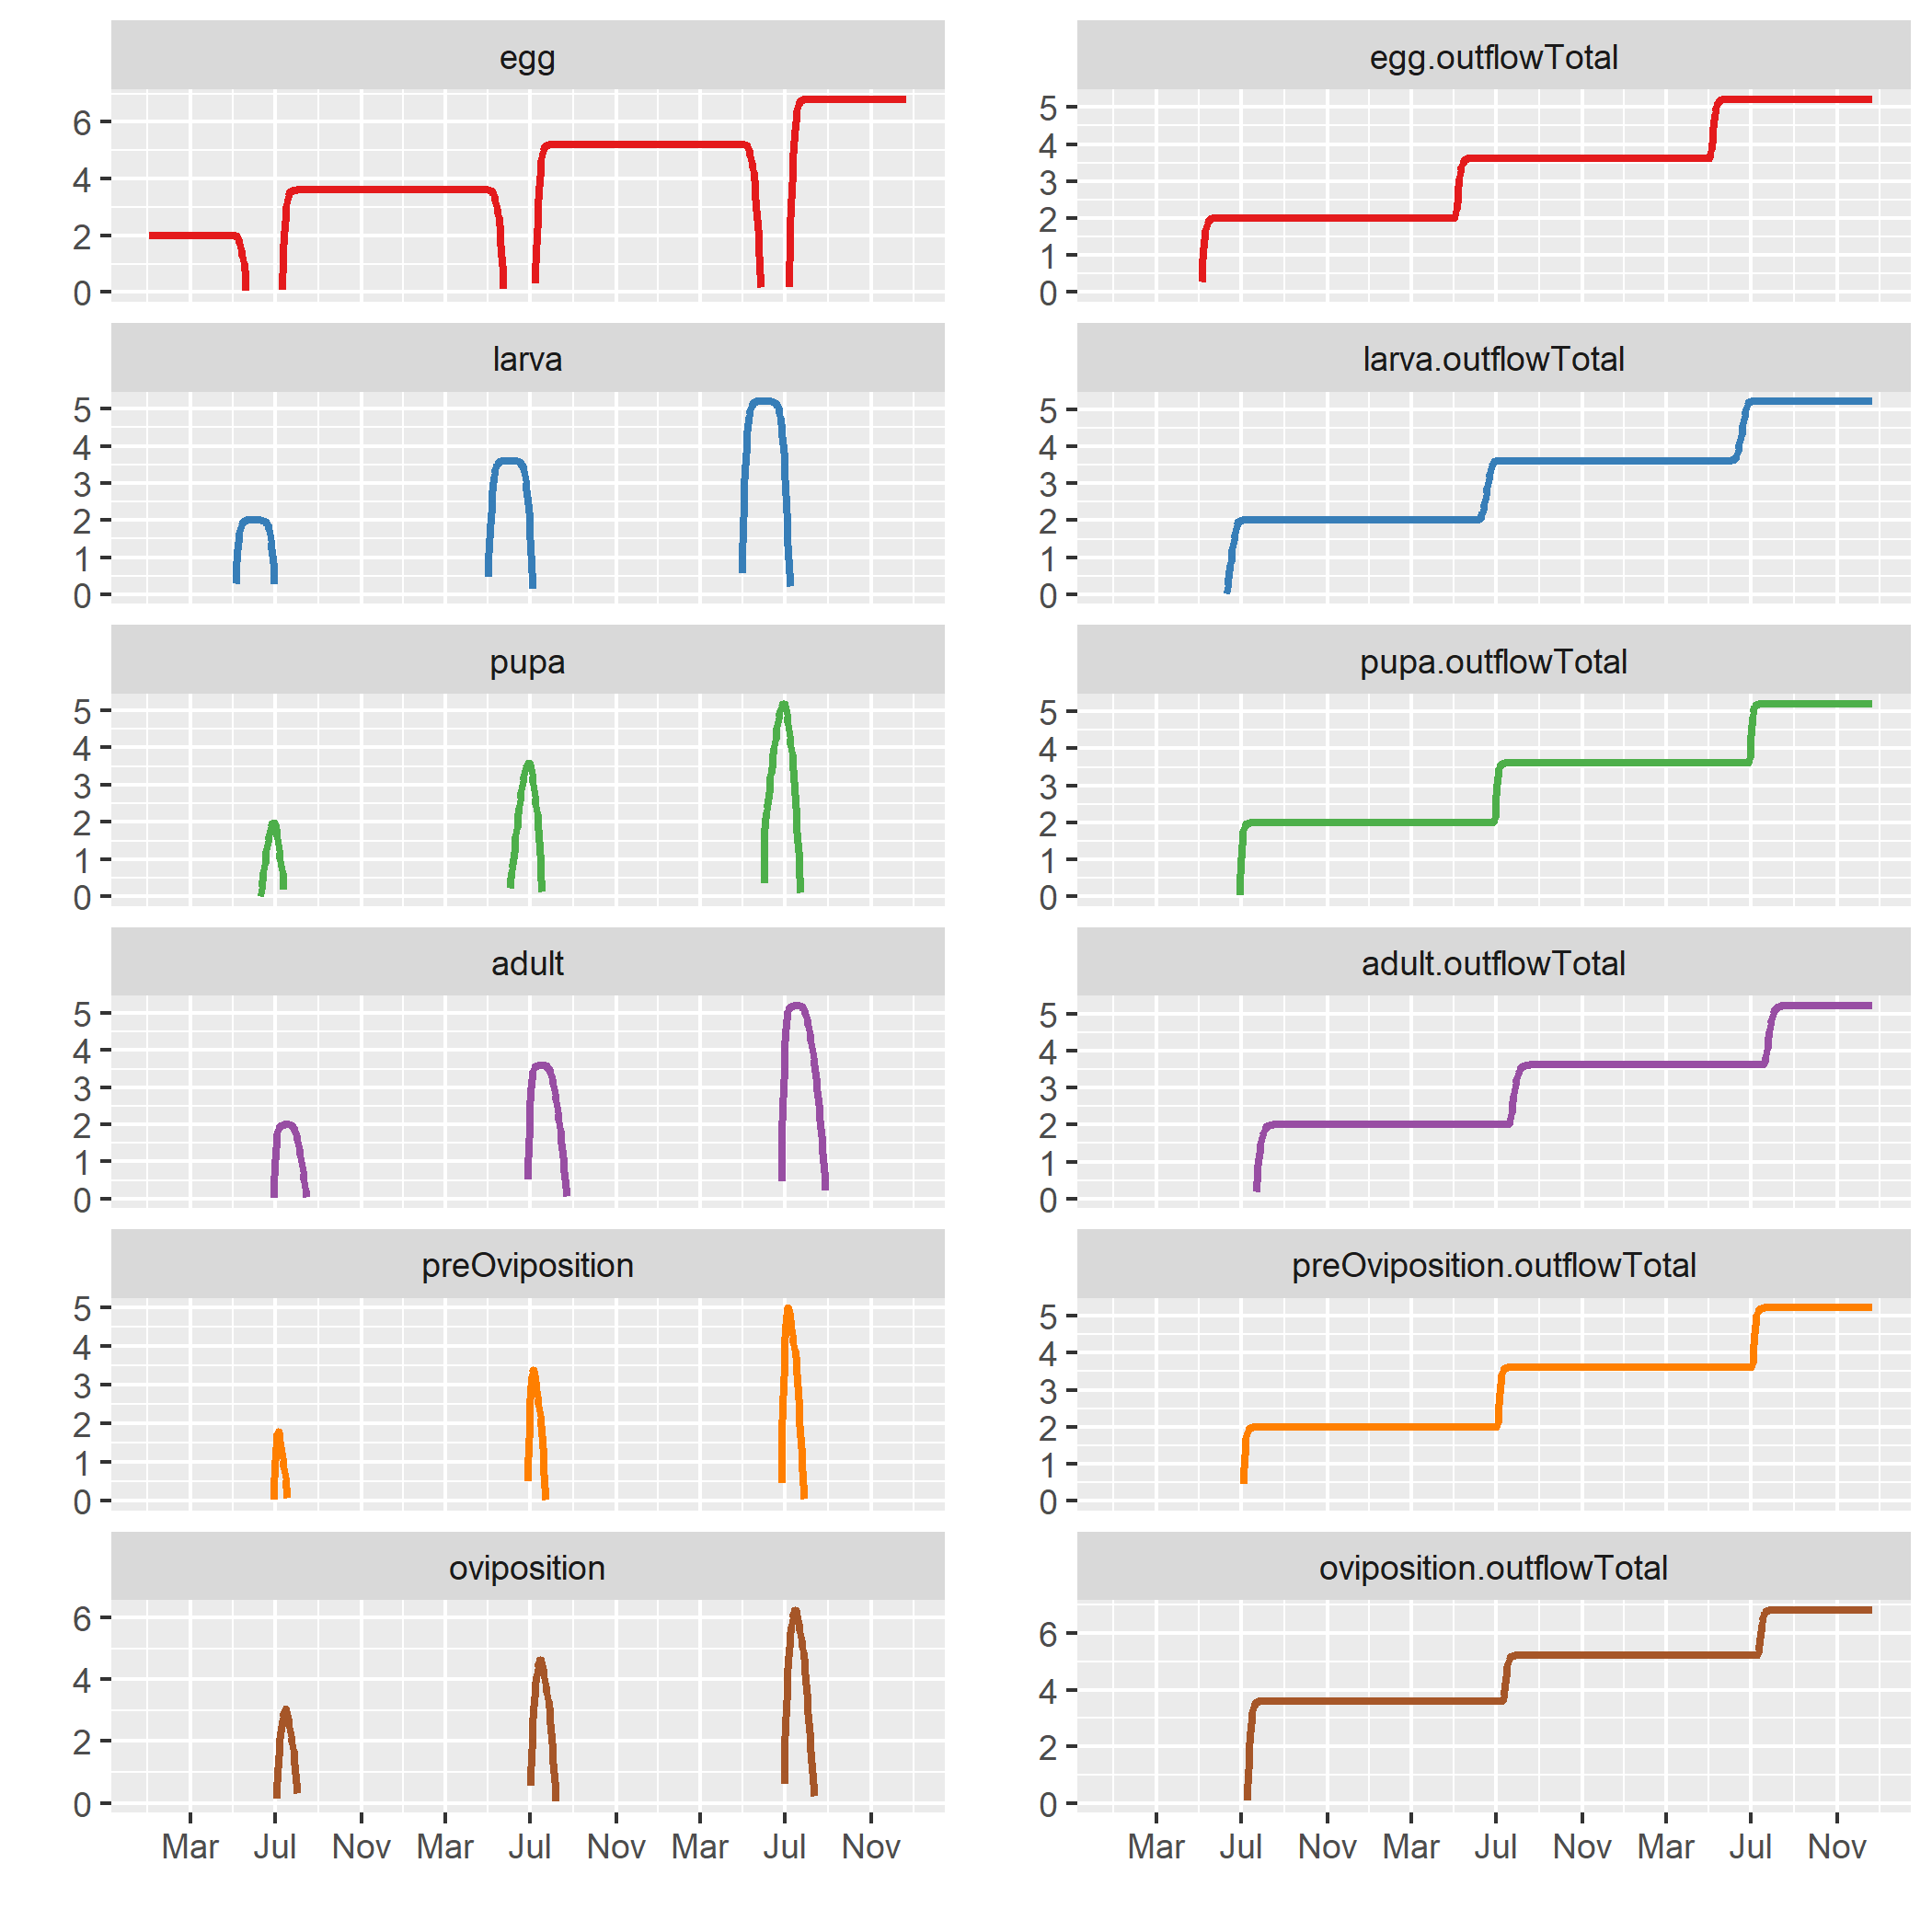
\includegraphics[width=\textwidth]{graphics/butterfly6}
\caption{Three years of life stage and oviposition phenology produced by the \filename{\inputfolder/book/butterfly6.box} script.}
\label{fig:butterfly6}
\end{figure}

\FloatBarrier
\section{A honeybee model}
The scientific literature on honeybees is enormous. There is plenty of information that can be used to build simulation models of various aspects of honeybee life. Here, we will limit ourselves to build a model of the population dynamics of a honeybee colony during one season in a temperate climate.

\subsection{Queen fecundity}
In a honeybee colony there is only one female laying eggs: the queen. Let's assume that her fecundity depends on day length only, increasing from 0 to 1,500 eggs per day, as day length increases from 8 to 12 hours.

To make certain that the fecundity sub-model works as expected, we will start out with a  script (\filename{\inputfolder/book/honeybee1.box}) that leaves out other components of the model:

\lstset{numbers=left}
\begin{boxscript}
// honeybee1.box
Simulation {
  .steps = dayLength[steps]
  SequenceByStep dayLength {
    .min = 5
    .max = 18
    .by = 1
  }
  ProportionalSignal fecundity {
    .input = dayLength[value]
    .minSignal = 0
    .maxSignal = 1500
    .threshold = 8
    .thresholdBand = 4
  }
  OutputR {
    Box p {
      &dayLength  = dayLength[value]
      &eggsPerDay = fecundity[value]
      &dottedLine = "geom_point(size=2)"
    }
    PageR {
      .width = 4
      .height = 2.5
      .xAxis = dayLength[value]
      PlotR {
        .ports = fecundity[value]
        .ggplot = p[dottedLine]
      }
    }
    PageR {
      .width = 4
      .height = 2.5
      .xAxis = p[dayLength]
      PlotR {
        .ports = p[eggsPerDay]
        .ggplot = p[dottedLine]
      }
    }
  }
}
\end{boxscript}
\lstset{numbers=none}

A \code{SequenceByStep} box is used to produce a linear series of numbers. For every \code{step} in the \code{Simulation}, it will produce the next value in the sequence. In this case, it goes from 5 (line 5) to 18 (line 6) by steps of length 1 (line 7). Hence, the output from this simulation, when represented as a data frame in R, will hold 14 rows with a \code{value} column running through the values 5, 6, \ldots, 17,18. A \code{SequenceByStep} box has an output \code{steps} which tells how many steps the simulation will need to go through to run through the whole sequence. This output is used as an input to the \code{Simulation} (line 3). Remember that in box scripts, children (\eg\ \code{dayLength}) are updated before parents (\eg\ the \code{Simulation} object), so the \code{Simulation} object will get this information in time.

\begin{figure} [b]
  \centering
  \begin{minipage}[b]{0.45\textwidth}
    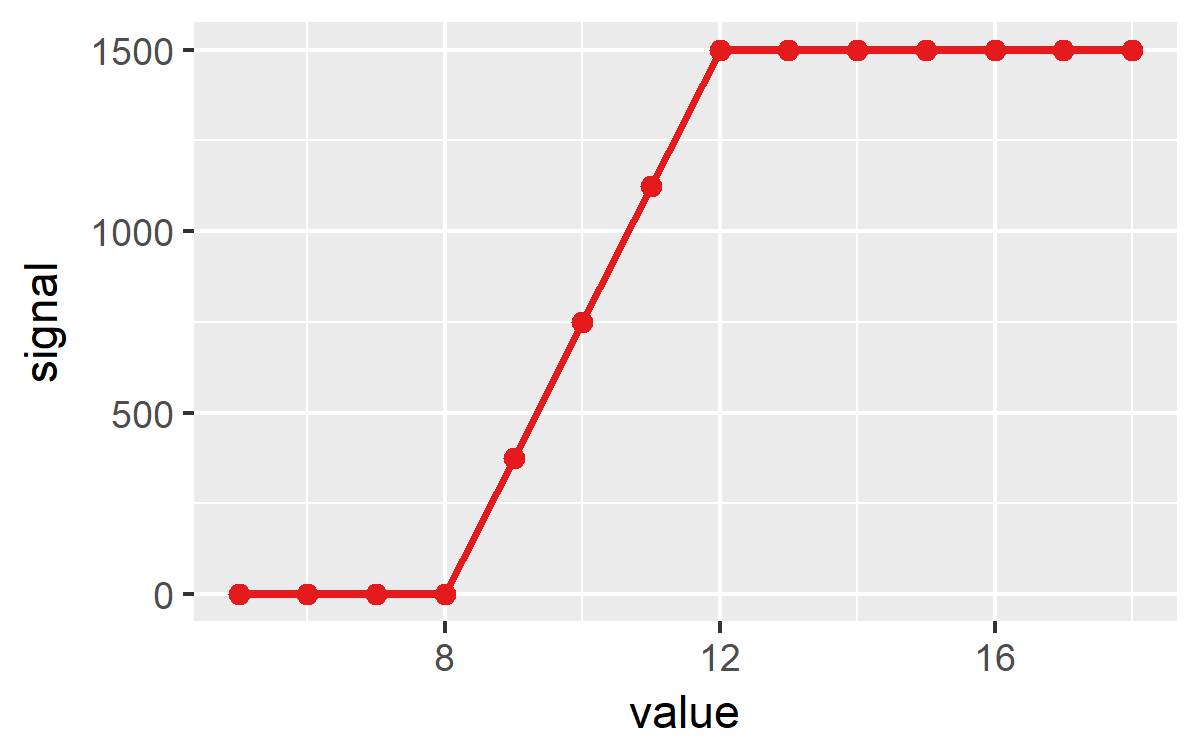
\includegraphics[width=\textwidth]{graphics/honeybee1-1}
  \end{minipage}
  \begin{minipage}[b]{0.45\textwidth}
    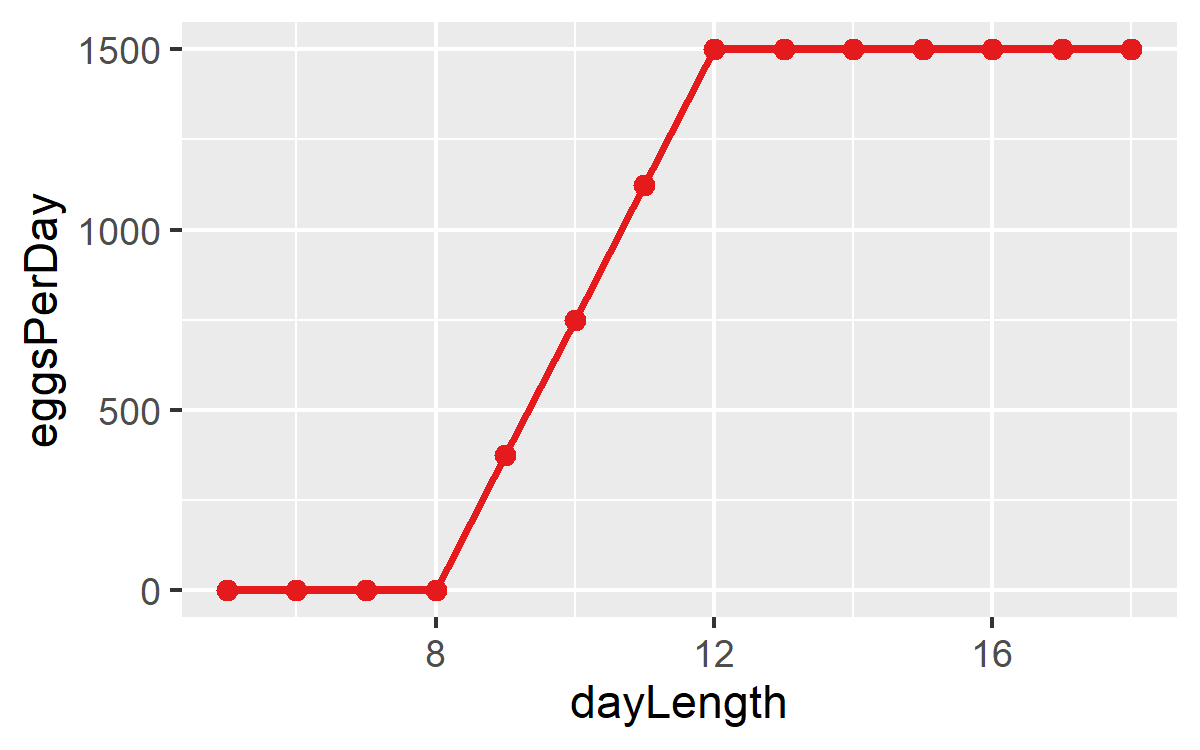
\includegraphics[width=\textwidth]{graphics/honeybee1-2}
  \end{minipage}
  \caption{Queen fecundity depending on day length with default (left) and improved (right) port names on axes. Generated by \filename{\inputfolder/book/honeybee1.box},}
  \label{fig:honeybee1}
\end{figure}

The \code{ProportionalSignal} box was originally developed as a building block to model process engineering with \US, but it turned out to be a versatile building block for rapid prototype modelling in general, \ie\ as a first approximation before caring for the details. It computes an output \code{value} based on minimum and maximum values (lines 11-12); the input names \code{minSignal} and \code{maxSignal} indicate  the engineering origin of this box. Its \code{value} changes linearly inside that range depending on the \code{input} (line 9). The linear slope begins at the input \code{threshold} (line 13) and spans over a width called the \code{thresholdBand} (line 14).

The plot (\iref{fig:honeybee1}) has been augmented with dots on top of the lines through the addition of a \code{geom_point} to the ggplot (lines 20, 28 and 37). The \code{dottedLine} is defined inside a box that we simply call \code{p} for brevity (and maybe lack of imagination). It is seen how fecundity changes with day length as expected. The two plots, produced by two different \code{PageR} objects (lines 22-30 and 31-39) are identical except for their axis labels. The plot on the right in \iref{fig:honeybee1} demonstrates the improved readability achieved by suitably named blind ports (lines 18-19), \code{dayLength} on the \xaxis\ and \code{eggsPerDay} on the \yaxis. The use of aptly named blind ports is a common practice for overruling default axis names.

In R you can also verify the output directly, if you take a look at the \code{sim} data frame:

\begin{rdialog}
> sim
iteration dayLength.value fecundity.value %\brk% dayLength eggsPerDay
1     5         5      0          0
1     6         6      0          0
1     7         7      0          0
1     8         8      0          0
1     9         9    375        375
1    10        10    750        750
1    11        11   1125       1125
1    12        12   1500       1500
1    13        13   1500       1500
1    14        14   1500       1500
1    15        15   1500       1500
1    16        16   1500       1500
1    17        17   1500       1500
1    18        18   1500       1500
> 
\end{rdialog}

In addition to the port outputs that you chose to produce the plots, there will always be an \code{iteration} column. This will contain all 1's, as in this case, when the model was run for only one iteration. This is determined by the \code{iteration} input to \code{Simulation} which defaults to a value of 1.

\subsection{Colony phenology}

The script for the complete model is not much longer than the previous script:

\lstset{numbers=left}
\begin{boxscript}
// honeybee2.box
Simulation sim {
  .steps = 365
  Calendar calendar {
    .initialDateTime = 1/1/2009
    .latitude = 60
  }
  Sun sun {
  }
  Box honeybee {
    Box queen {
      ProportionalSignal fecundity {
        .input = sun[dayLength]
        .minSignal = 0
        .maxSignal = 1500
        .threshold = 8
        .thresholdBand = 4
      }
    }
    Stage egg {
      .inflow = ../queen/fecundity[value]
      .duration = 5
    }
    Stage larva {
      .inflow = ../egg[outflow]
      .duration = 14
    }
    Stage pupa {
      .inflow = ../larva[outflow]
      .duration = 3
    }
    Stage worker {
      .inflow = ../pupa[outflow]
      .duration = 28
    }
  }
  OutputR {
    Box p {
      &eggsPerDay = queen/fecundity[value]
    }
    PageR {
      .xAxis = calendar[date]
      PlotR {
        .ports = sun[dayLength] |
                   p[eggsPerDay] |
                   *[content] 
        .ggplot = "scale_x_datetime( 
                     breaks = date_breaks('months'), 
                     labels = date_format('%\%%b') 
                    )"
      }
    }
  }
}
\end{boxscript}
\lstset{numbers=none}

The \code{fecundity} sub-model is  unchanged (lines 12-18), except that the \code{input} is now taken from the \code{sun} object (line 13). Astronomocally, day length depends on date and latitude. Here, we simulate a whole year (lines 3 and 5) at \ang{60} northern latitude (line 6). A \code{Sun} box defaults to import date and latitude from the \code{calender} box. You can check this by typing

\begin{rdialog}
> help Sun
\end{rdialog}

Laid eggs are directed to the \code{inflow} port of the \code{egg} stage from where they trickle through subsequent life stages, following the same paradigm as for the butterfly model previously. Honeybees maintain constant temperature for the immature stages, which makes a day scale more appropriate than a day-degree scale.

The output (\iref{fig:honeybee2}) shows the expected dynamics through the year. The number of workers become stable as the daily inflow into the stage (from the pupa stage) matches the outflow (due to life length expiration). The density reached for workers is quite realistic, 42,000, as we can find in R:

\begin{rdialog}
> max(sim$worker.content)
[1] 42000
> 
\end{rdialog}

We will leave the model at this stage although much remains to be done. For instance, workers produced in the autumn are so-called 'winter bees' with much longer life span than the workers produced earlier in the year. For that we would need to include a \code{winterBee} box, and we would need to direct the eggs laid to either the \code{worker} or the \code{winterBee} box depending on, \eg\ day length.


\begin{figure}
\centering
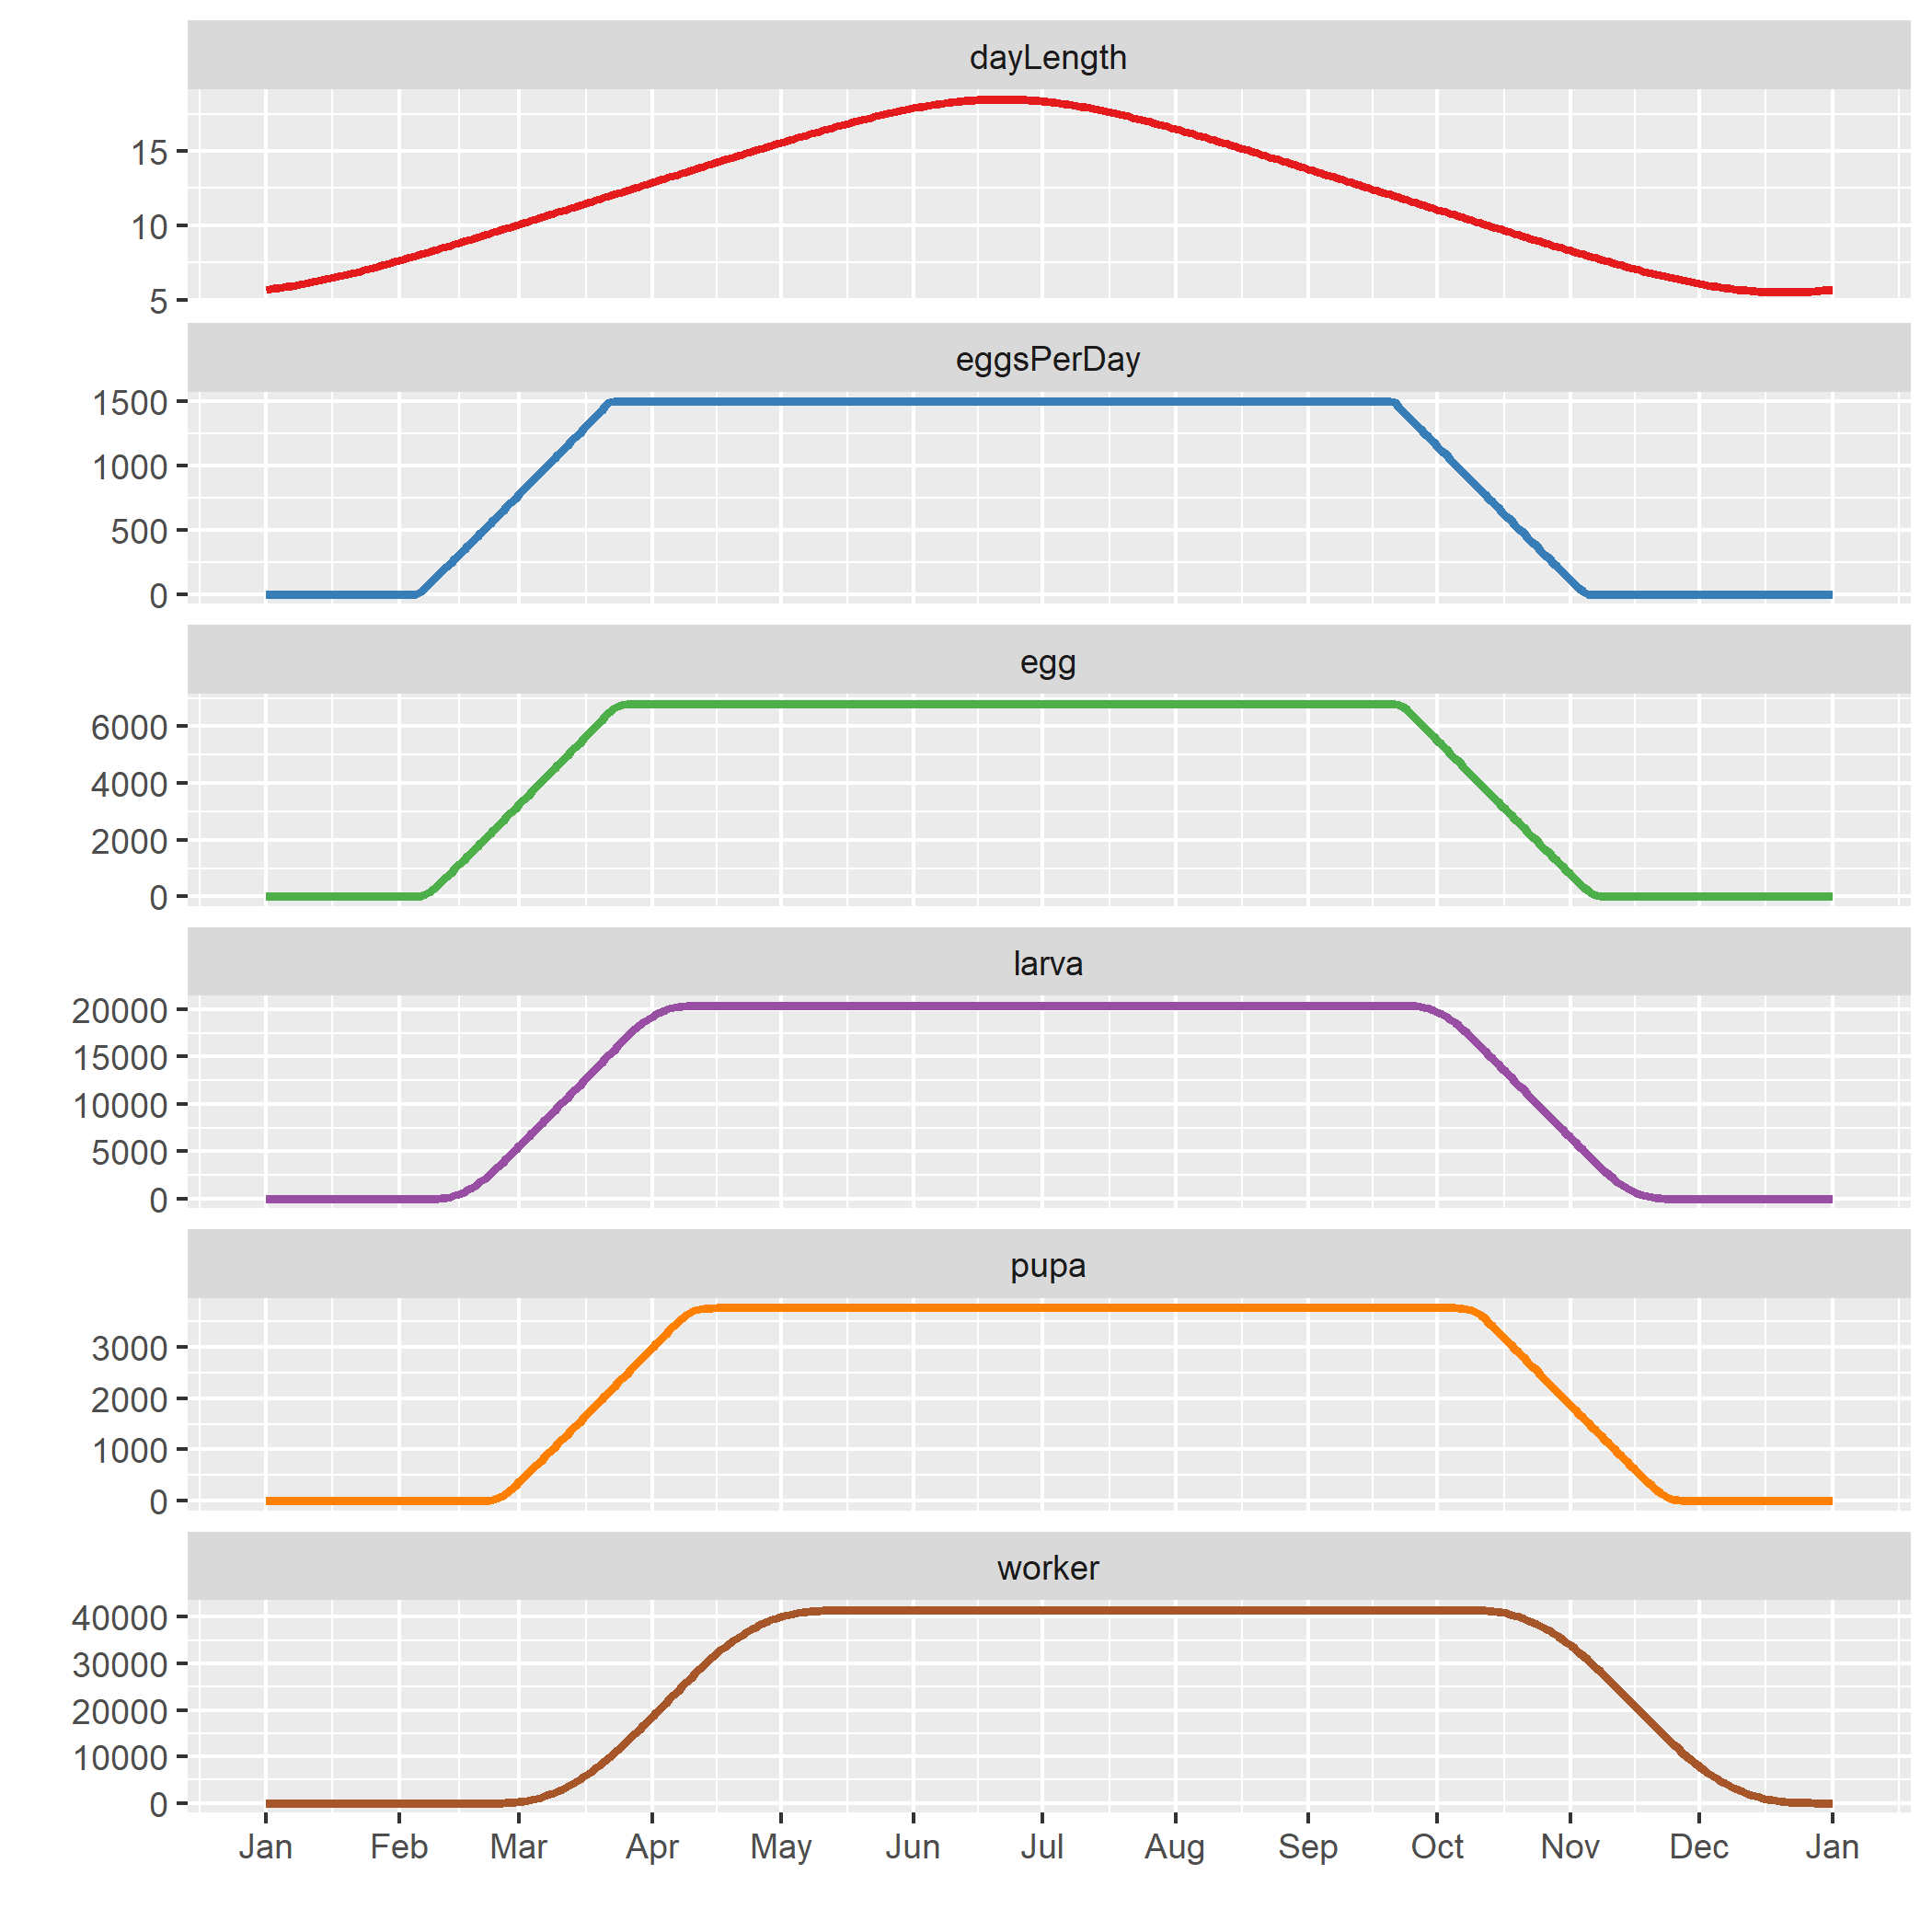
\includegraphics[width=\textwidth]{graphics/honeybee2}
\caption{Colony phenology driven by day length. Generated by \filename{\inputfolder/book/honeybee2.box}.}
\label{fig:honeybee2}
\end{figure}
